
\section{Diagonalization of a symmetric $2\times 2$ matrix}

From \url{http://scipp.ucsc.edu/~haber/ph116A/diag2x2_11.pdf}



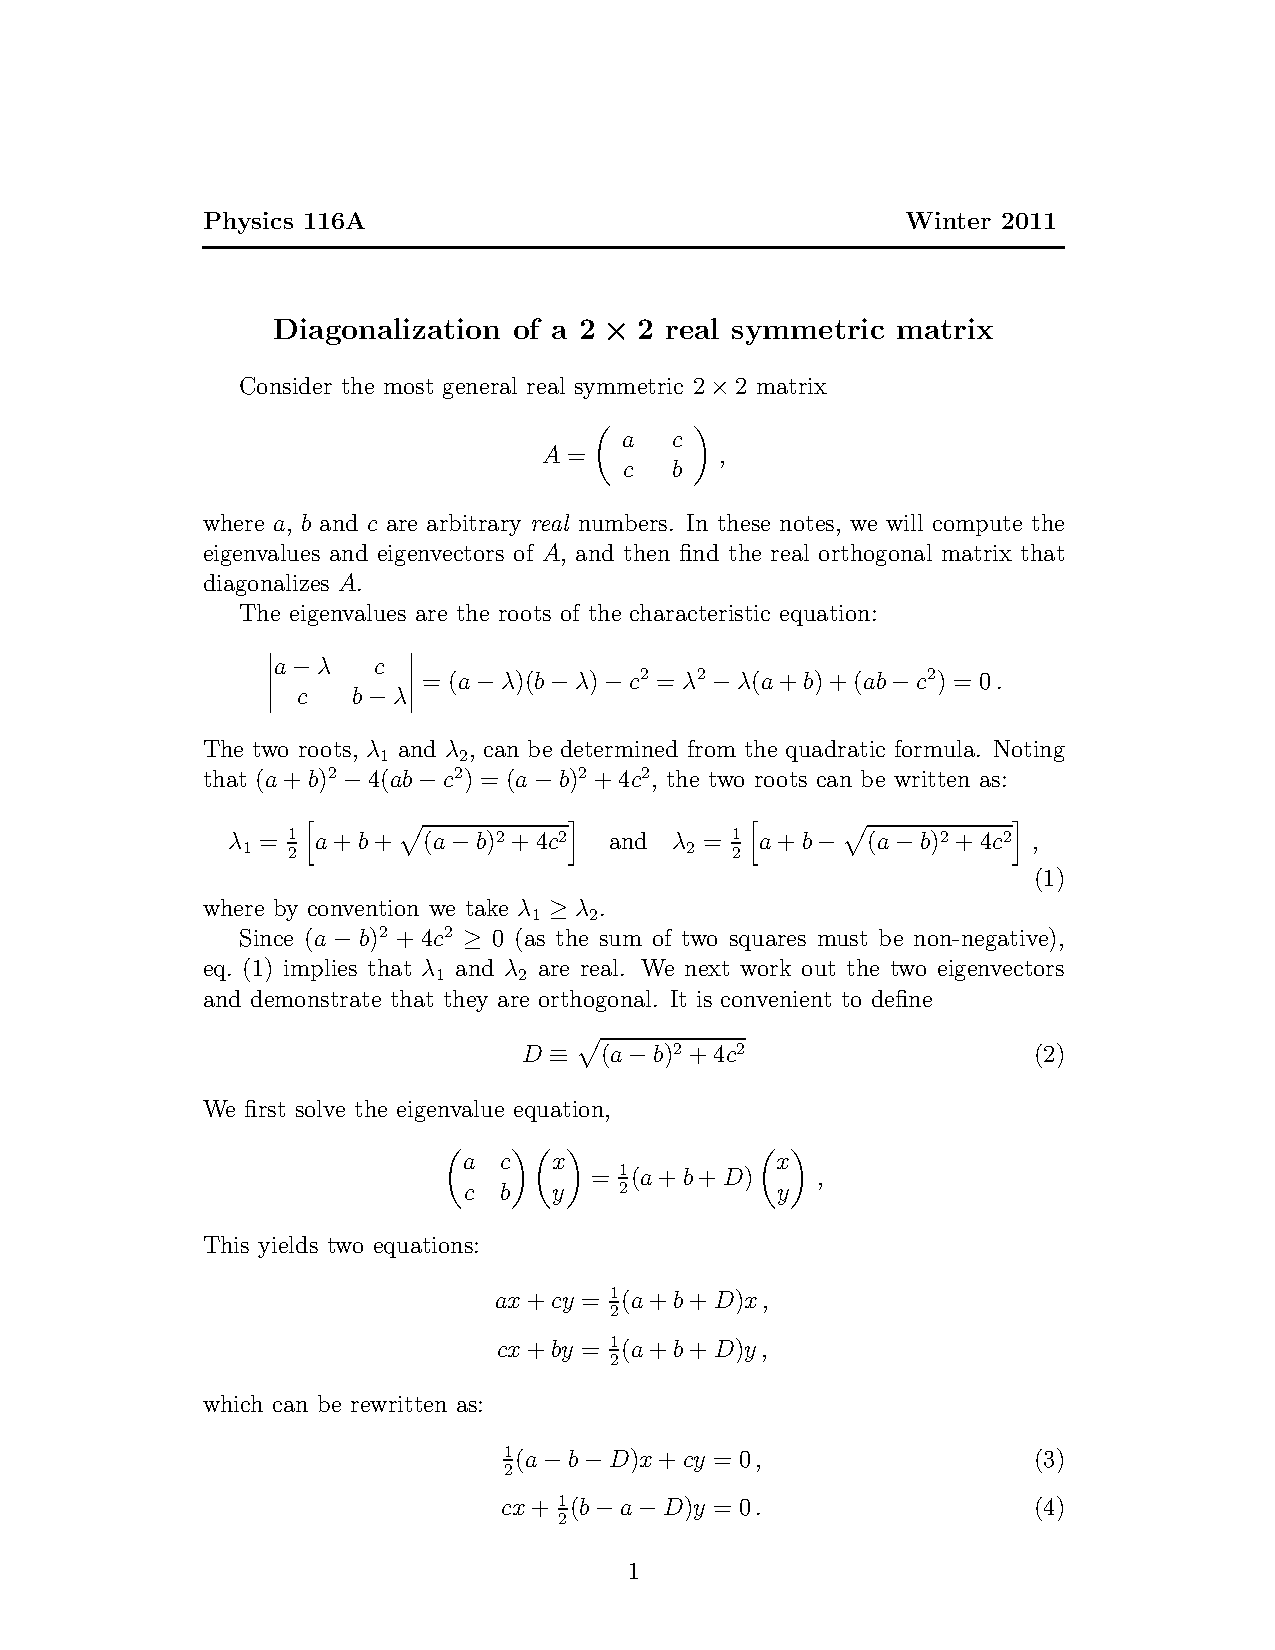
\includepdf[pages=-]{diag2x2.pdf}

From the eigenvalue equations (1) we can easily check that in addition to trace invariance, we have that 
\begin{align}
  \lambda_1-\lambda_2=\sqrt{\left( a-b \right)^2-4c^2}\,.
\end{align}
Replacing back in eq. (9)
\begin{align}
  \sin2\theta=\frac{2c}{\lambda_1-\lambda_2}\,.
\end{align}


%%% Local Variables: 
%%% mode: latex
%%% TeX-master: "beyond"
%%% End: